\section{Increase in the number of critical paths}
\label{sec:criticalpaths}

The increased variance in delay caused by near-threshold operation is directly responsible for an increase in the number of critical paths.
A critical path can be defined as any path that has a high probability of exceeding a given clock \cite{Wang:2004bw}.
For our case of trying to find the maximum frequency a given device can run, we can instead consider a critical path as a path that has a high probability of setting FMAX; that is, of being the slowest path in the system.
  
Consider a distribution of the nominal delays of paths within a chip (Figure~\ref{fig:normal}).
In the case of no variations, clock speed is set by the path with the highest nominal delay.
Once delay variation is added in, however, points that are close in delay to the path with the highest nominal delay could act instead as the critical path in a portion of chips.
This means that it is any path that falls within $n\frac{\sigma_v}{\mu}$ of the maximum nominal delay for a given $n$ that is set by the design where $\sigma_v$ is the standard deviation and $\mu$ is the mean of the timing path variation distribution.
The number of critical paths then becomes the area under this delay-count curve where the delay is greater than $n\frac{\sigma_v}{\mu}$
 
\begin{figure}[thpb]
    \centering
    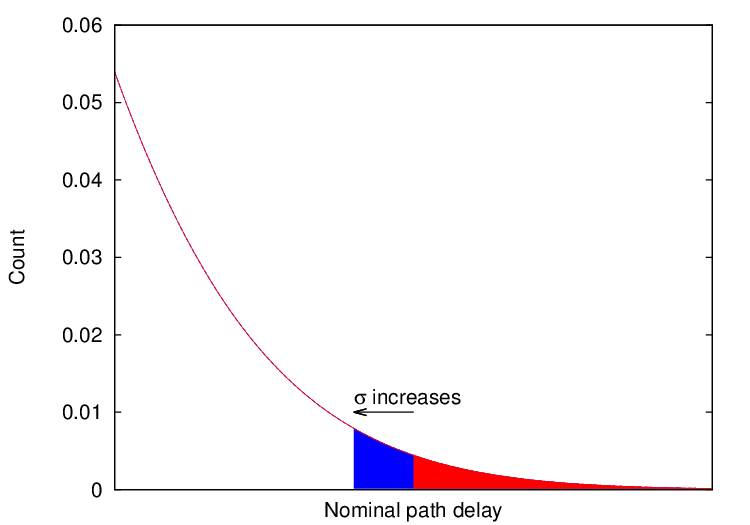
\includegraphics[width=0.4\textwidth]{normal.png}
    \caption{As $\sigma_v$ increases, the number of critical paths (shaded area) increases}
    \label{fig:normal}
\end{figure}
 
 Although the shape of the nominal delay distribution will vary depending on the design of the chip, if it is assumed this shape is strictly convex, it can be shown that the number of critical paths $N_{cp}$ increases at least linearly with $\sigma_v$.
Considering that $\frac{\sigma_v}{\mu}$ increases approximately 7x as the voltage drops into the near-threshold regime, there is at least a 7x increase in the number of critical paths.
This will translate into a reduction in the maximum frequency of the design\cite{Bowman:2002cp} and added design complexity, as more critical paths will have to be optimized.

